\documentclass{standalone}
\usepackage{tikz}
\definecolor{lpurple}{HTML}{c9b5c8}
\definecolor{lred}{HTML}{e1e9ef}
\definecolor{lyellow}{HTML}{e1e9ef}

\begin{document}

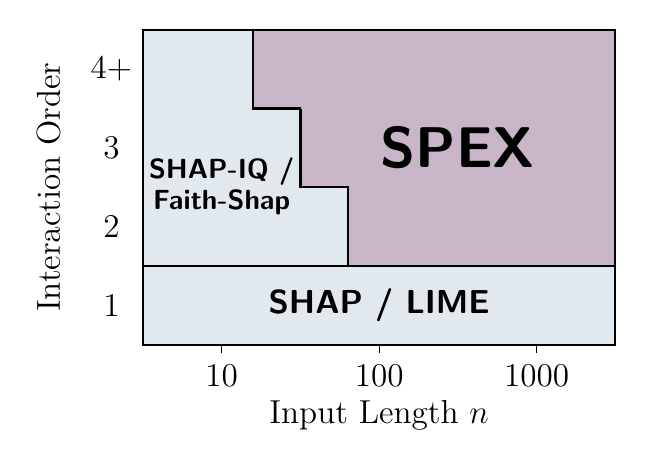
\begin{tikzpicture}
    \node at (3, -0.9) {\large Input Length $n$};
    \node[rotate=90] at (-1.2, 2) {\large Interaction Order};

    % X-axis labels
    \node at (1, -0.4) {\large 10};
    \node at (3, -0.4) {\large 100};
    \node at (5, -0.4) {\large 1000};
    \draw (1,0) -- (1,-0.1);
    \draw (3,0) -- (3,-0.1);
    \draw (5,0) -- (5,-0.1);

    % Y-axis labels (flipped order)
    \node at (-0.4, 3.5) {\large 4+};
    \node at (-0.4, 2.5) {\large 3};
    \node at (-0.4, 1.5) {\large 2};
    \node at (-0.4, 0.5) {\large 1};

    \fill[lpurple] (0,0) rectangle (6,4);

    % SHAP/LIME Region (adjusted for flipped axis)
    \fill[lred] (0,0) rectangle (6,1);
    
    \fill[lyellow] (0,1) rectangle (2.6,2.001);
    \fill[lyellow] (0,2) rectangle (2,3.002);
    \fill[lyellow] (0,3) rectangle (1.4,4);

    % Divider Lines
    \draw[thick] (0,0) -- (6.0125,0);
    \draw[thick] (0,-0.0125) -- (0,4.0125);
    \draw[thick] (0,1) -- (6,1);
    \draw[thick] (6,0) -- (6,4);
    \draw[thick] (0,4) -- (6.0125,4);
    
    \draw[thick] (1.4,3) -- (1.4,4);
    \draw[thick] (1.987,2) -- (2.6125,2);
    \draw[thick] (2.013,3) -- (1.3875,3);
    \draw[thick] (2,2) -- (2,3);
    \draw[thick] (2.6,1) -- (2,1);
    \draw[thick] (2.6,1) -- (2.6,2);
    \draw[thick] (6,1) -- (2.6,1);

    \node[font=\sffamily] at (3, 0.5) {\large \textbf{SHAP / LIME}};

    \node[font=\sffamily] at (1, 2.2) { \textbf{SHAP-IQ /}};
    \node[font=\sffamily] at (1, 1.8) { \textbf{Faith-Shap}};

    \node[font=\sffamily, color=black] at (4, 2.5) {\huge\textbf{SPEX}};

\end{tikzpicture}

\end{document}
